\documentclass{standalone}
\usepackage{mathpazo}
\usepackage[american]{circuitikz}

\begin{document}
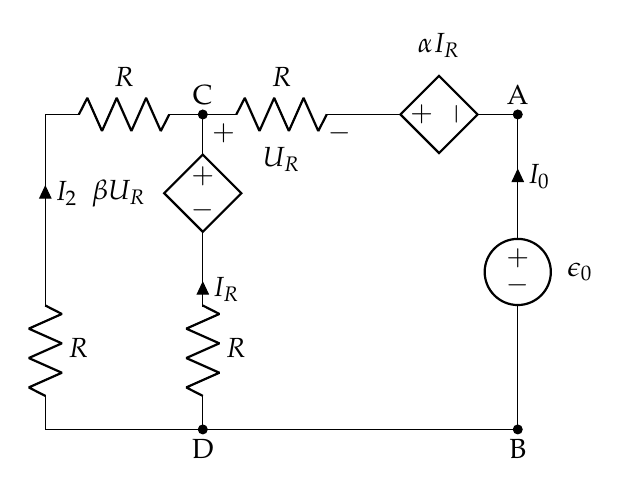
\begin{tikzpicture}
  \coordinate (A) at (0,4);
  \coordinate (B) at (2,4);
  \coordinate (C) at (6,4);
  \coordinate (E) at (0,0);
  \coordinate (F) at (2,0);
  \coordinate (G) at (6,0);
  \draw
  (A) to [R, l = $R$, -*] (B)
  to [R, l = $R$, v = $U_R$] ++(2,0)
  to [cV, -*, v=$\alpha I_R$] (C) node[above] {A};
  \draw
  (A) to [short, i<= $I_2$] ++(0,-2) to [R, l=$R$] (E);
  \draw
  (B) node[above] {C} to [cV, v_=$\beta U_R$] ++(0,-2) to [R, l=$R$, i<= $I_R$] (F) node[below] {D};
  \draw
  (E) to [short, -*] (F) to [short, -*] (G) node[below] {B};
  \draw
  (C) to [V, v=$\epsilon_0$, i = $I_0$] (G);
\end{tikzpicture}
\end{document}